%%%%
\newpage
\section{Black Carbon}

Apesar da importância do BC nos problemas ambientais atmosféricos, há muita 
ambiguidade em seu tratamento, começando pelo modo como é denominado e seguindo
pelas propriedades das partículas, faltando precisão aos termos a ele 
relacionados (soot, BC, BS, EC, ou fuligem, negro de fumo, fumaça preta, 
carbono elementar, em português). \citet{petzold2013}, dentre outros trabalhos, 
destacam que, desta forma, termos como BC e EC referem-se a um conjunto de 
materiais cujas propriedades não estão bem definidas e ressaltam que material 
carbonáceo na atmosfera ocorre como misturas muito variáveis de compostos de 
carbono, com diferentes propriedades. Sugere, assim, definir o BC a partir de 
um conjunto de propriedades, compreendendo uma microestrutura similar à grafite,
uma morfologia fractal com cadeias de nanoesferas agregadas, um material 
refratário que volatiliza em torno de 4000K, gaseificando-se apenas por oxidação
em temperaturas acima de 340 $\degree$ C, não sendo solúvel em água ou qualquer
outro solventes. O trabalho de análise e revisão organizado pela OMS, 
\citet{janssen2012}, destaca que esse carbono pode ser carvão - que origina-se 
de processos de pirólise (como na queima de biomassa), tendo cor mais próxima do
castanho - ou fuligem, de cor negra e formada sob combustão em altas 
temperaturas, como ocorre nos motores diesel. A análise TOT consegue 
diferenciá-los. A EPA-US também gerou um relatório sobre BC \citep{epa2012} com
a contribuição de algumas dezenas de autores. Realizou uma ampla revisão e 
discussão sobre BC, caracterizando-o extensivamente e tratando de seus efeitos 
na saúde e o meio ambiente, particularmente no que diz respeito ao clima, 
avaliando inclusive medidas mitigatórias para controlá-lo. 
Apresenta imagens bastante ilustrativas, tanto sobre a geração quanto às suas 
características micro e macroscópicas.

Todos esses trabalhos relacionam métodos de medida de BC, que preconizam medidas
absolutas, como TOT ou TOR,  ou relativa, como aqueles baseados na absorção de 
luz visível pelo material em suspensão na atmosfera ou coletado sobre filtros. 
Esse segundo método é incomparavelmente mais simples e de menor custo que os 
primeiros. Nós optamos por empregar medidas por refletância. Neste caso pode-se 
usar os mesmos filtros da análise elementar por XRF-ED (PTFE ou policarbonato), 
pois ambas técnicas são não destrutivas. Todas operações envolvidas nas medições
por refletância consomem algo em torno de um a dois minuto, em média, 
possibilitando a determinação de diversas centenas de amostras em poucos dias.
De um modo geral isso também é interessante numa perspectiva de avaliação de 
séries históricas, já que BC pode ser correlacionado com Black Smoke (BS), 
uma medida que órgãos de controle ambiental costumam realizar há muitos anos 
por refletância. \citet{quincey2007} e \citet{heal2012} discutem relações entre 
estas medidas, destacando que em Londres, por exemplo, elas são feitas desde 
1920. Mas alertam, entretanto para o cuidado que se deve ter já que a estrutura 
de BC,EC e OC, acompanha as diferenças ou mudanças de característica regionais 
e temporais do aerossol e precisam ser contemporizadas.

Também há registros históricos de medidas relativas de BC realizadas desde 
1980 por Aetalômetro, técnica que incide um feixe colimado de luz monocromática 
sobre o filtro com amostra coletada medindo-se a quantidade de luz abosorvida
por atenuação \citep{targino2016}. 

Thermal Optical-Reflectance (TOR) ou Thermal-Optical Transmittance (TOT), 
fornecem medidas absolutas de EC e OC, mas são destrutivas e necessitam de um 
filtro especial e de aparatos de medidas e amostragem exclusivos, 
tendo custo bem mais elevado.

%%%%
\subsection{Refletância}

Concentrações de BC foram obtidas por refletômetro do tipo 
\textit{Smoke Stain Reflectometer} modelo EEL43D da empresa Diffusion System, 
que devido à sua simplicidade, é tradicionalmente usado para medidas de BC em 
amostras ambientais \citep{lack2014}. A técnica baseia-se na alta seção 
de choque de absorção de luz pelo BC, na região do visível, e assume que 
toda absorção é devida ao BC presente na amostra.

\begin{figure}[H]
  \centering
  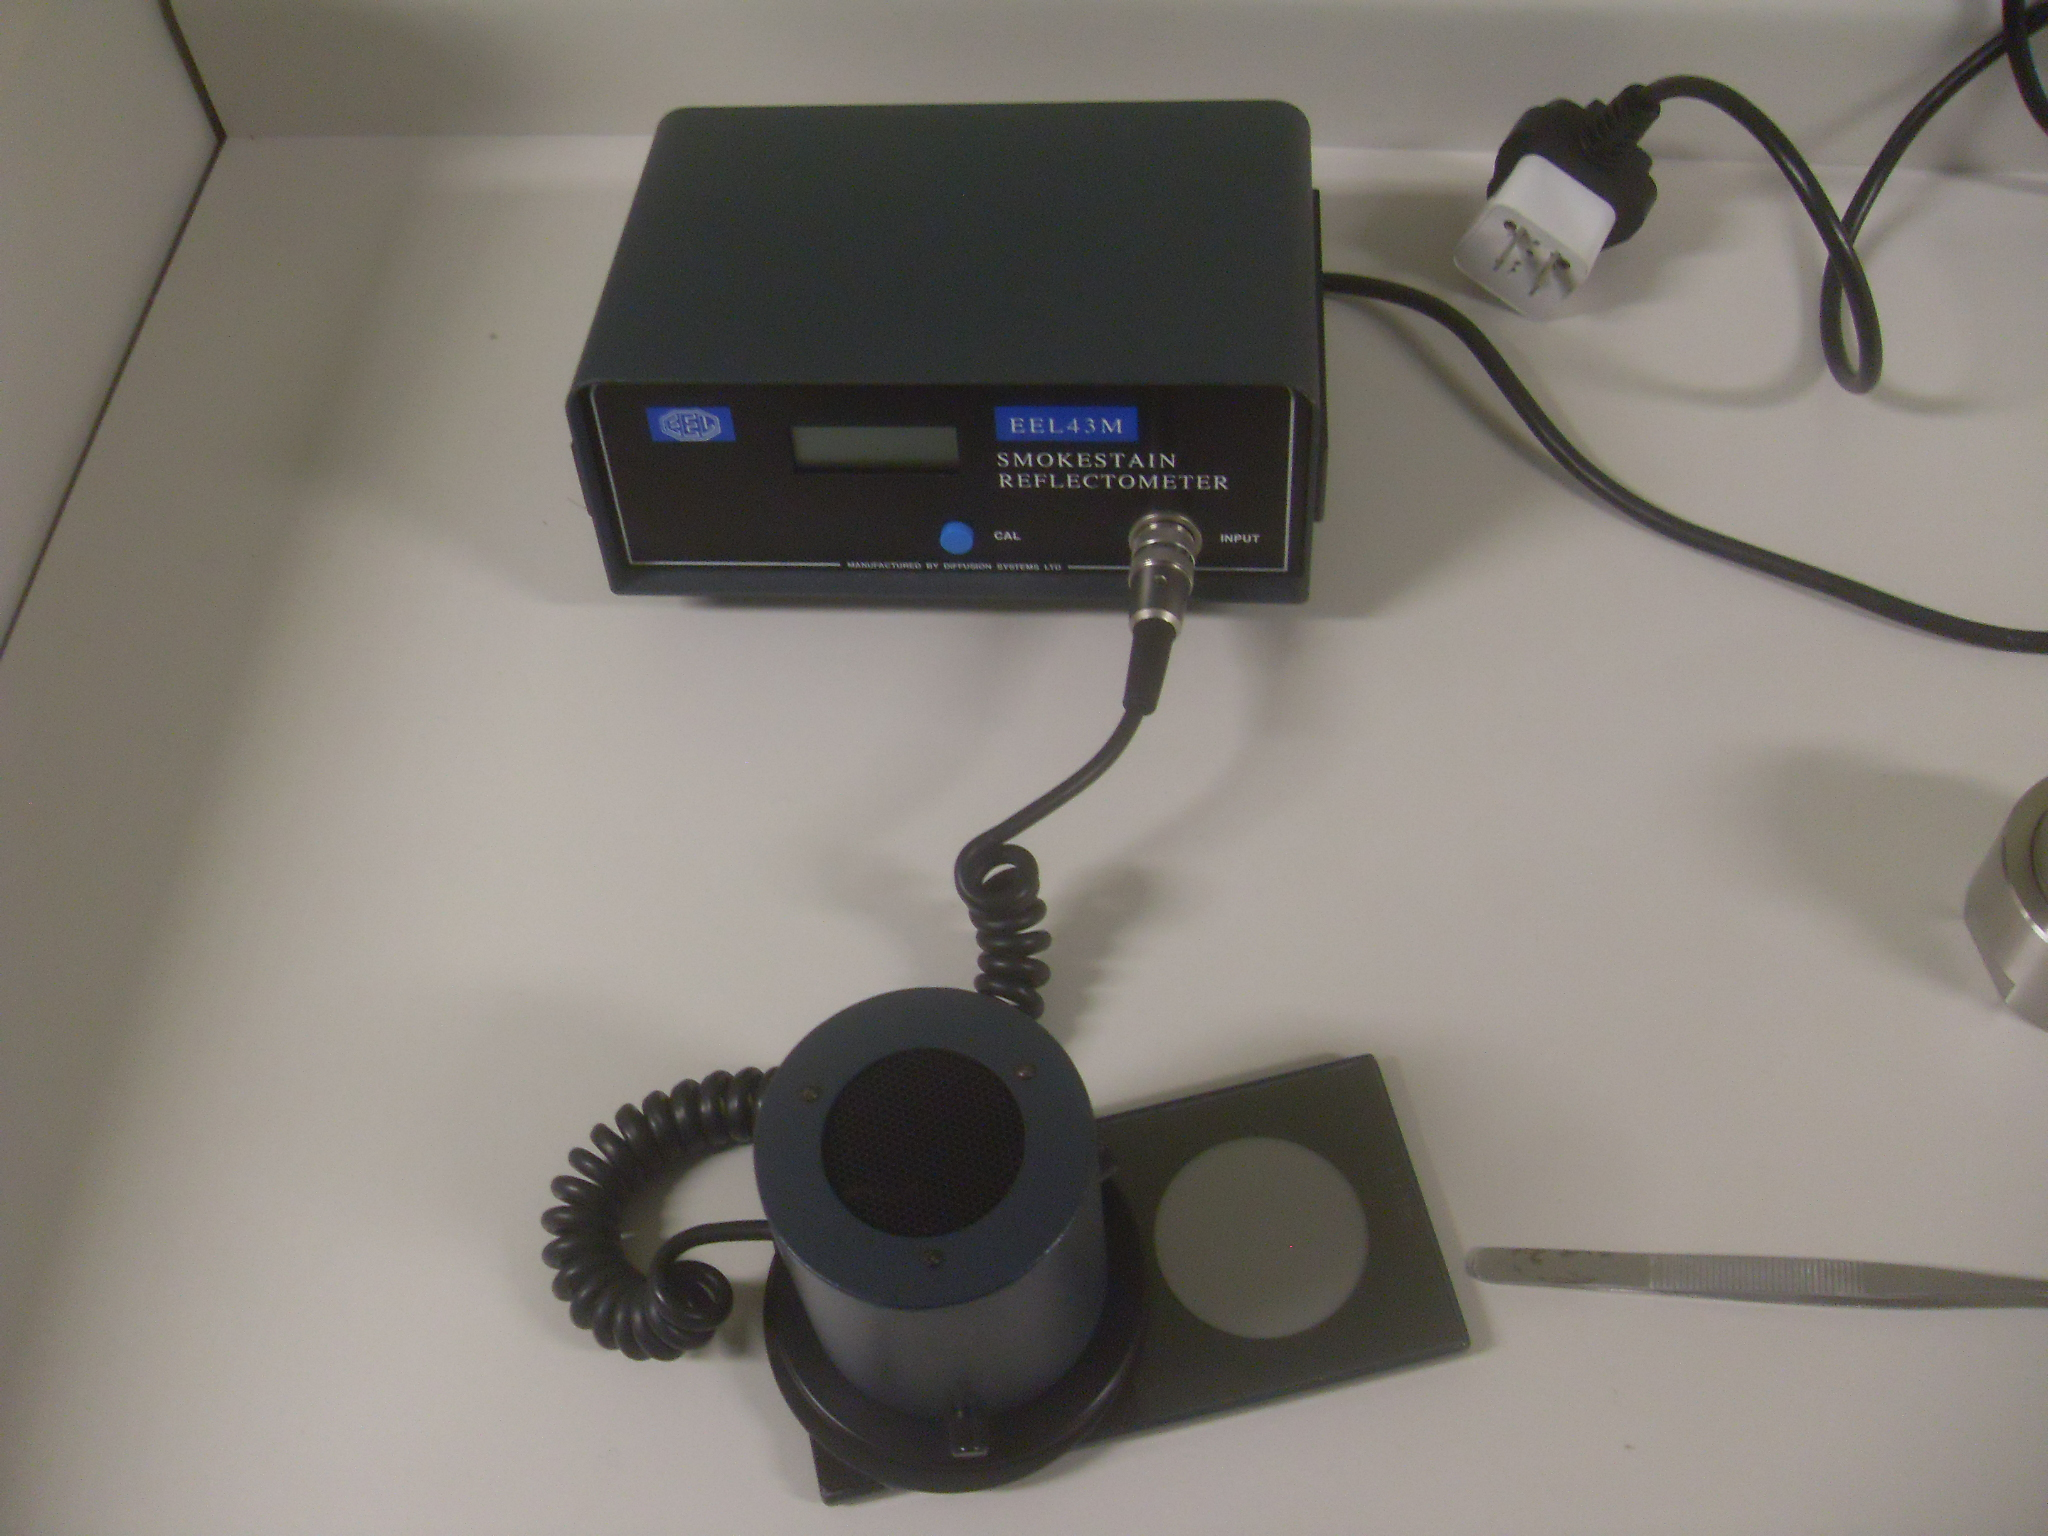
\includegraphics[width=0.5\textwidth]{../inputs/images/refletometro.jpg}
  \caption{Refletômetro da Diffusion System modelo ELL43D 
           e peças auxiliares de fixação no LAPAt}
\end{figure}

Na refletância, uma área definida da amostra é ilumindada por lâmpada de 
tungsténio, sendo parte da luz incidente absorvida pelas partículas do 
filtro e parte refletida. Uma fotocélula com orifício circular, localizada
entre a lâmpada e a amostra, mede a porcentagem da luz refletida (I).
Um filtro branco é usado para fixar o 100\% das leituras a cada 3 medidas.

A absorção de luz que atravessa um meio com coeficiente de absorção ($\alpha$) 
homogêneo, segue um processo clássico. A intensidade I da luz em um ponto x da
amostra (meio) homogênea, decai $-dI$ ao atravessar uma espessura $dx$, 
sendo o decaimento diretamente proporcional a I:

\begin{equation}
  \label{eq:dIdx}
   \frac{dI}{dx} = -\alpha I
\end{equation}

fazendo-se a separação das variáveis, pode-se integrar os dois lados da equação:

\begin{equation}
  \int_{I_0}^{I} \frac{dI}{I} = - \int_{0}^{D} \alpha dx
\end{equation}

Resultando em uma relação exponencial entre o decaimento da intensidade do feixe
de luz incidente ($I_0$) e a intensidade transmitida ($I$), 
em função da espessura (D) da amostra:

\begin{equation}
  \label{eq:I_BC}
  I = I_0 \cdot exp(-\alpha D)
\end{equation}

No caso da refletância o feixe de luz vai e volta pela amostra, ficando:

\begin{equation}
  \label{eq:I_BC2}
  I = I_0 \cdot exp(-\alpha 2D)
\end{equation}

O detector opera sobre uma área fixa e, assim, a medida que nos interessa é a 
massa por unidade de área (A). Ao ser multiplicada pela área total de amostragem
no filtro ela fornece a massa total coletada. A massa $m$ que o detetor observa 
é $m = \rho \cdot V = \rho \cdot D \dot A$, onde $\rho$ é a densidade da amostra. 
Podemos usar esta relação para substituir $D$ na equação \ref{eq:I_BC2}, 
ficando:

\begin{equation}
  \label{m/a}
  I = I_0 \cdot exp \left( -\frac{2\alpha}{\rho}.\frac{m}{A} \right)
\end{equation}

Aplicando-se logarítimo nos dois lados da equação e rearranjando os termos, 
obtemos:

\begin{equation}
  \label{m/a_2}
  \frac{m}{A} = K \cdot (2-logI) 
\end{equation}

onde $\frac{1}{K} = 2 \cdot \frac{\alpha}{\rho} \cdot log(e)$
é uma constante e usou-se que $I_0$=100\%, sendo $log 100$ = 2.

A relação linear entre $\frac{m}{A}$ e log($I$) oferece bom ajuste empírico 
quando se trabalha com BC, permitindo a calibração do equipamento. 
Ressalve-se haver uma perda de linearidade para valores muito baixos de 
refletância (amostras muito carregadas).  

%%%%
\subsection{Thermal Optical Transmittance}

Apresenta-se apenas os fundamentos gerais do TOT, pois o empregamos apenas para
calibrar o método de refletância. As medidas de TOT foram realizadas por outros
integrantes do projeto geral de pesquisa.
O TOT é um método absoluto para medir carbono orgânico (OC) e 
carbono elementar (EC) e baseia-se no fato de que ambos convertem-se para gás 
em diferentes temperaturas e condições de oxidação \citep{birch1998}.

Aquecendo-se a amostra paulatinamente em ambiente não oxidante (presença de He),
ocorre progressiva volatização dos compostos orgânicos nas temperaturas mais 
baixas. A evaporação do carbono elementar ocorre acima de 580 $\degree C$.
Durante a fase de volatilização do OC, parte dele sofre pirólise, 
convertendo-se em EC e aumentando a concentração deste componente na amostra. 
Um sistema ótico com feixe de laser de intensidade controlada, registra este 
acúmulo em função da perda de transmitância da amostra.
Na fase de volatização do EC, contabiliza-se como OC, todo o EC extraído da 
amostra até o ponto em que o sistema óptico indique ter sido retomada a sua 
transmitância original. Daí em diante é que se passa a contabilizar o EC 
originalmente presente na amostra.
Faz-se a medida do C, oxidando-o para $CO_2$ ao passar por uma placa de dióxido
de magnésio aquecida, que segue por um catalizador de níquel, 
onde o dióxido de carbono é reduzido a metano $CH_4$. O $CH_4$ é quantificado 
com uma detector do tipo Flame Ionization Detector.
Para análises TOT é necessário fazer a coleta em filtros de quartzo, aumentando 
os custos e tornando mais complexa a logística das medidas, 
pois é necessário montar ponto de medida paralelos aos da coleta para análise
elementar.
